\section{Raytracing}
 
\begin{figure}[H]\centering
    \subfloat[]{
        \hspace*{0.05\textwidth}
         \includegraphics[width=0.3\textwidth]{images/mouille.jpg}
    \label{fig:shadowmap3}
    }
    \hspace*{0.1\textwidth}
    \subfloat[ ]{
    \includegraphics[width=0.5\textwidth]{images/vray.png}
    \label{fig:shadowmap1}
    }
   \end{figure}


\begin{figure}[H]\centering
    \subfloat[]{
        \hspace*{0.05\textwidth}
         \includegraphics[width=0.4\textwidth]{images/freestyle.jpg}
    \label{fig:shadowmap3}
    }
    \hspace*{0.1\textwidth}
    \subfloat[]{
    \includegraphics[width=0.4\textwidth]{images/pixar.jpg}
    \label{fig:shadowmap1}
    }
   \end{figure}





\subsection{Raytracing Algorithmen}
 \begin{figure}[H]
    \centering
    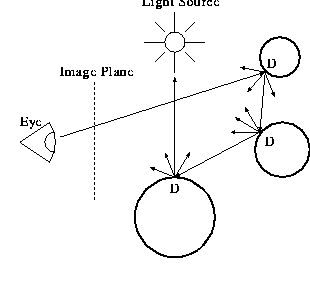
\includegraphics[width=0.75\textwidth]{images/rayTracing.png}
    \caption{Strahlenverfolgung}
    \label{fig:diffus}
\end{figure}

 
\subsubsection{Die Rendergleichung (Erste und zweite Form)}

Durch Hinzunahme des von dem Oberflächenpunkt emittierten Lichtes $L_e(x, \omega_o)$ zu dem   an diesem Punkt reflektiert Lichtes erhalten wir die sogenannte Renderingleichung 
\begin{align}
L_o(x, \omega_o) = L_e(x, \omega_o)  + \displaystyle \int_{H^2}f_r (x, \omega, \omega_0) \cdot L_i(x, \omega)  \cdot  \cos(\theta) d\omega \; ,
\end{align}
wobei $L_e(x, \omega_o)$ die von der Oberfläche emittierte Strahlungsleistung ist. 

\begin{Bemerkung}
Für transparente Oberflächen muss über $S^2$ integriert werden.
\end{Bemerkung}
Definiert man die Menge $\Omega$  als die Menge aller Flächen  in der Szene und
\begin{align}
V(x,y) := \begin{cases}
1 \text{ falls } \overline{xy} \cap (\Omega -\{x,y\}) = \emptyset \\
0 \text{ sonst }
\end{cases}
\end{align}
so ist $L_i(x, \omega_y) = V(x,y) \cdot L_o(y, \omega_x)$ (Energieerhaltung).
Zusammen mit der Beziehung 
\begin{align}
d\omega =  \frac{1}{||x -y||^2} \cdot  \cos(\theta_y) dA_y
\end{align}
 und der Definition 
\begin{align}
G(x,y) := V(x,y)  \frac{ \cos(\theta_x) \cdot  \cos(\theta_y)}{||x -y||^2} 
\end{align}
erhält man die Rendergleichung in zweiter Form 
\begin{align}
L_o(x, \omega_o) = L_e(x, \omega_o)  + \displaystyle \int_{\Omega} f_r (x, \overline{xy}, \omega_o) \cdot   L_o(y, \overline{xy})  \cdot  G(x,y) \cdot   dA_y \; .
\end{align} 

\subsubsection{Pfadformulierung der Rendergleichung}
Definiert man den sogenannten Transport  Operator
\begin{align}
(T \circ  L)(x, \omega) :=  \displaystyle \int_{H^2}f_r (x, \omega, \omega_0) \cdot L(x, \omega)  \cdot  \cos(\theta) d\omega \; ,
\end{align}
so lässt sich die Rendergleichung schreiben als
\begin{align}
L = L_e + T \circ L \; .
\end{align}
oder mit der Identitätsabbildung $id$ als
\begin{align}
L_e = (id - T) \circ L \; .
\end{align}
Wir erhalten damit 
\begin{align}
L = (id - T)^{-1} \circ L_e \; .
\end{align}
wobei 
\begin{align}
 (id - T)^{-1}= \sum_{i= 0}^{\infty} T^i  \; .
\end{align}
eine konvergente Reihe ist, falls $f_r (x, \omega, \omega_0) < 1$ gilt. Letztere Bedingung bedeutet anschaulich,  dass kein Material perfekt reflektierend ist. Die Gleichung ist eine Verallgemeinerung der geometrischen Reihe auf Operatoren.
 
\subsection{Raycasting}
\subsection{"Klassisches" Raytracing}
Das klassische Raytracing nach Whitted ist durch folgenden rekursiven Algorithmus gegeben:
\begin{itemize}
\item 
\end{itemize}

\subsection{BRDF-Shader}
 \begin{figure}[H]
    \centering
    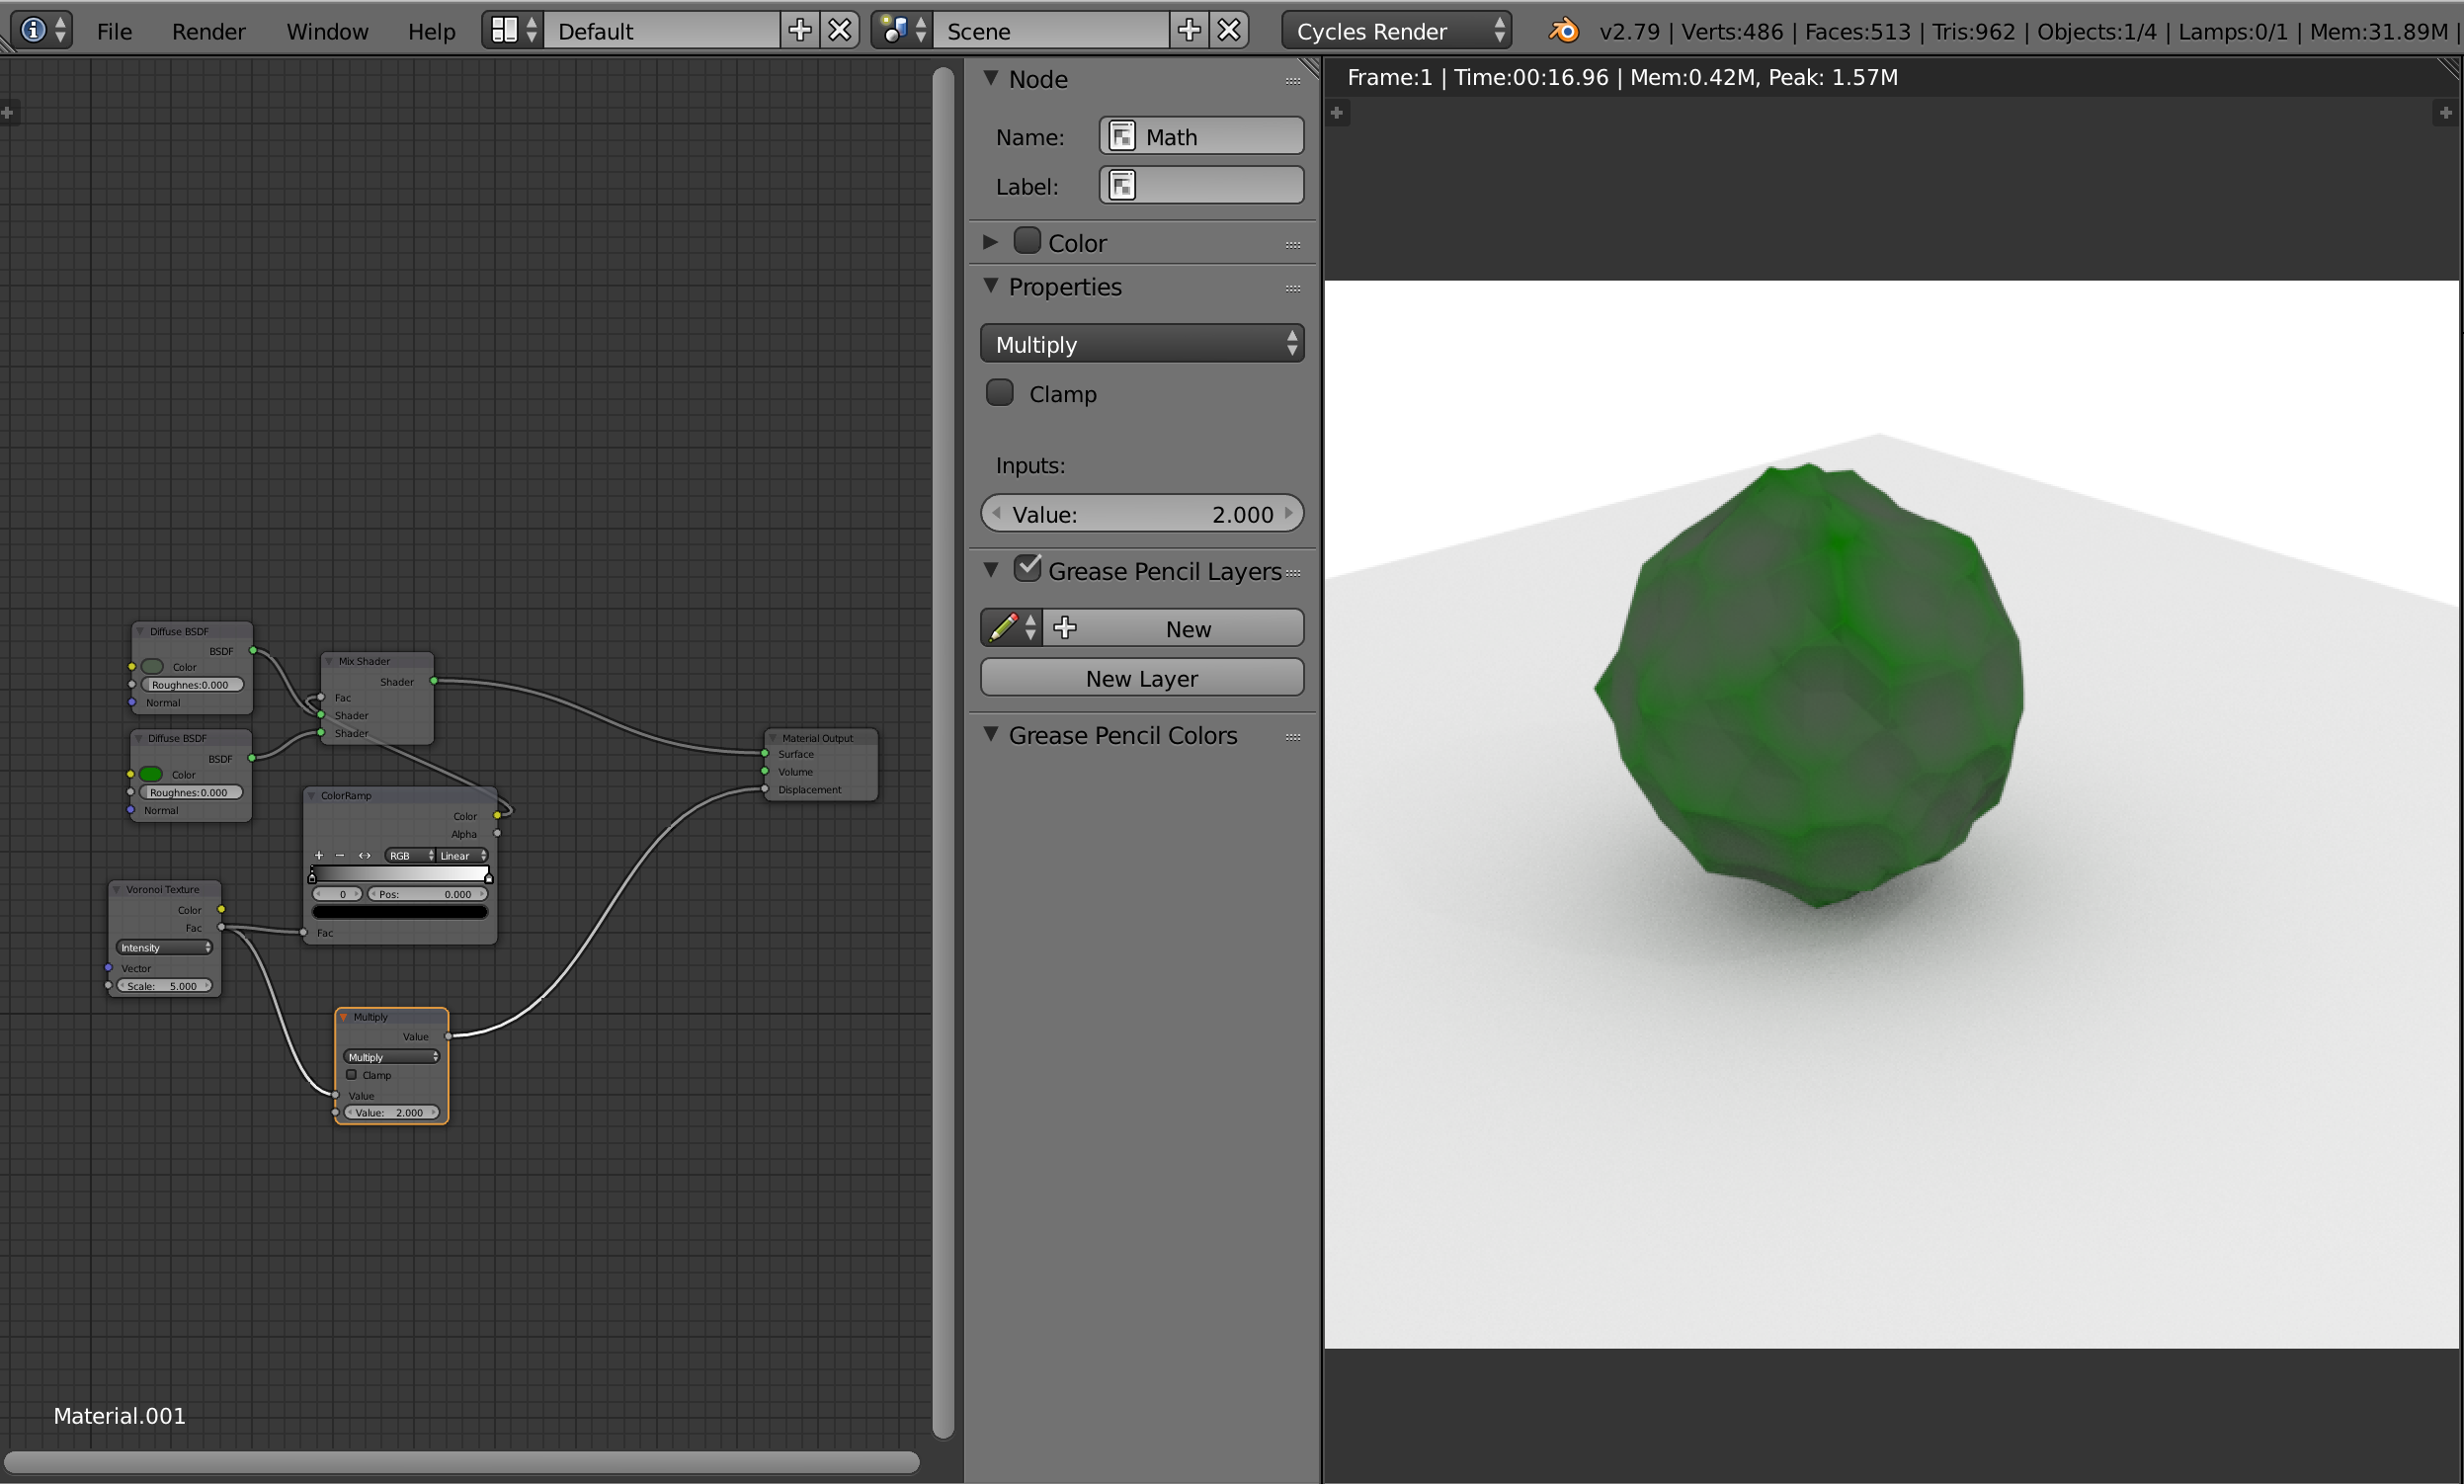
\includegraphics[width=0.95\textwidth]{images/blender_noodle.png}
    \caption{Grafische BRDF-Shader Programmierung in Blender}
    \label{fig:diffus}
\end{figure}
 \begin{figure}[H]
    \centering
    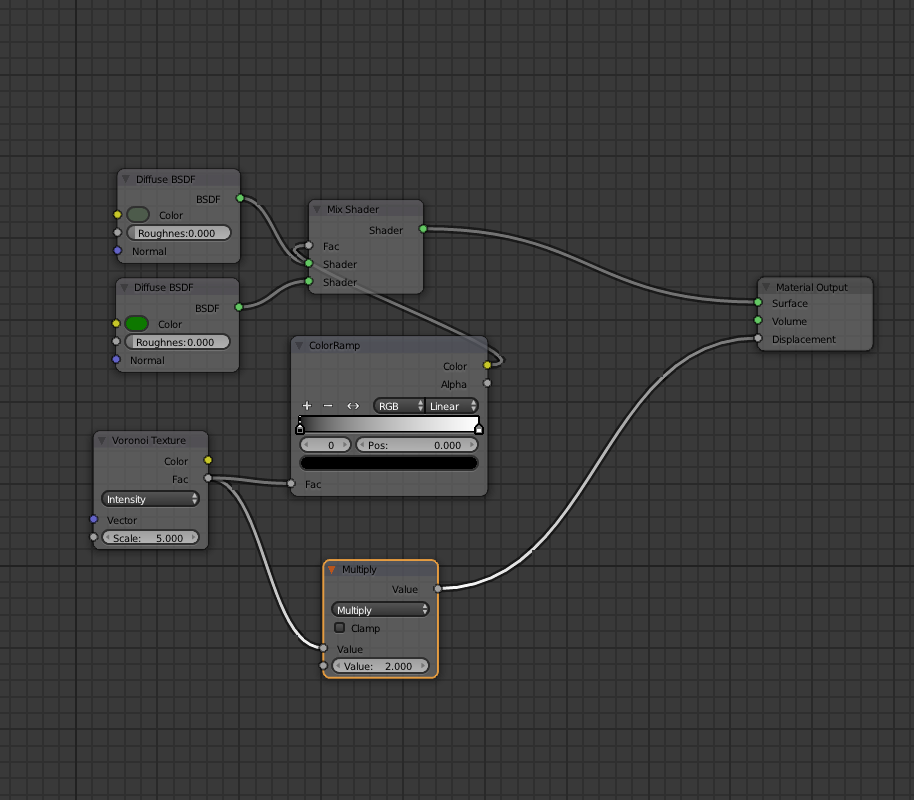
\includegraphics[width=0.75\textwidth]{images/blender_noodle2.png}
    \caption{Grafische BRDF-Shader Programmierung in Blender}
    \label{fig:diffus}
\end{figure}

\subsection{Radiosity Verfahren}
Das Radiosity Verfahren löst die Rendergleichung näherungsweise im Fall rein diffuser Oberflächen beziehungsweise rein Lambertscher Strahler. In diesem Fall sind  $L(x, \omega) = L(x)$ und $ f_r (x, \omega, \omega') = f(x)$ konstant  für alle  Richtungen $\omega$ und $\omega'$ und  mit der daraus resultierenden Beziehung  
\begin{align}
B(x) & = \int_{H^2} L(x) \cos{\theta} d\omega \\
\Leftrightarrow B(x) & =  L(x) \underbrace{\int_{H^2} \cos{\theta} d\omega}_{= \pi} \\
\Leftrightarrow \frac{B(x)}{\pi} & = L(x) \;.
\end{align}
erhält man durch Einsetzen in die Rendergleichung die Radiosity Gleichung
\begin{align}
B_o(x)   -B_e(x) - f (x) \cdot  \displaystyle \int_{\Omega}   B_o(y) \cdot G(x,y) \cdot   dA_y    =  0\; . 
\end{align}

Eine Möglichkeit diese approximativ zu lösen ist die Galerkin-Methode, die eine Näherungsweise Lösung dieses Problem auf die Lösung eines linearen Gleichungssystem reduziert.
Hierzu unterteilt (approximiert) man  alle  Oberflächen  in $\Omega$ mit endlich vielen planeren Flachenstücken $F_i$, welche auch  Patches genannt werden.
Des weiteren definiert man die sogenannten Basisfunktionen 
\begin{align}
\phi_i(x) := \begin{cases}
1 \text{ falls } x \in F_i \\
0 \text{ sonst}
\end{cases}
\end{align}
und Approximiert alle beteiligten Funktionen durch Linearkombinationen dieser Funktionen, was zu der Gleichung 
\begin{align}
\sum_i B_i \phi_i    =  \sum_i E_i  \phi_i +  ( \sum_i f_i \phi_i)  \cdot  \sum_i \displaystyle \int_{F_i}    B_i \phi_i   \cdot G(x,y) \cdot   dA_y   
\end{align}
führt. Multipliziert man beide Seiten mit $\phi_j$ und Integriert anschliessend beide Seiten über $F_j$  erhält man die diskrete Radiosity Gleichung
\begin{align}
B_j     =  E_j    +  f_j \sum_i    F_{ji} \cdot B_i \;  ,
\end{align}
wobei $A_j$ der Flächeninhalt des Patches $F_j$ und 
\begin{align}
F_{ji} := \frac{1}{A_j}\displaystyle \int_{F_j}  \displaystyle \int_{F_i}   G(x,y) \cdot   dA_y 
\end{align}
 ist.  Dies führt auf das lineare Gleichungssystem $M \cdot B = E$ mit 
\begin{align}
M &:= (m_{ij}) \text{ mit } m_{ij} = \begin{cases} 1- f_i \cdot F_{ij}  \text{ für } i = j \\  - f_i \cdot F_{ij} \text{ sonst} \end{cases} \\
B &:= \begin{pmatrix} B_1 \\ \vdots \\ B_n
\end{pmatrix} \\
E &:= \begin{pmatrix} E_1 \\ \vdots \\ E_n
\end{pmatrix}
\end{align}



 \begin{figure}[H]
    \centering
    \includegraphics[width=0.7\textwidth]{images/radiosity_process.jpg}
    \caption{Patches und Übertragung der Lichtenergie zwischen einzelnen Patches}
    \label{fig:diffus}
\end{figure}

 \begin{figure}[H]
    \centering
    \includegraphics[width=0.7\textwidth]{images/diffus.png}
    \caption{Rendering der Cornell Box mit rein diffusem Beleuchtungsmodell}
    \label{fig:diffus}
\end{figure}

 \begin{figure}[H]
    \centering
    \includegraphics[width=0.7\textwidth]{images/Radiosity_Comparison.jpg}
    \caption{Direkte Beleuchtung im Vergleich mit dem Radiosity Verfaren.l}
    \label{fig:diffus}
\end{figure}
\subsection{Monte-Carlo Raytracing und Pathtracing}


\begin{figure}[H]\centering
    \subfloat[Rendering der Cornell Box mit Pathtracing und wenig Samples]{
        \hspace*{0.05\textwidth}
    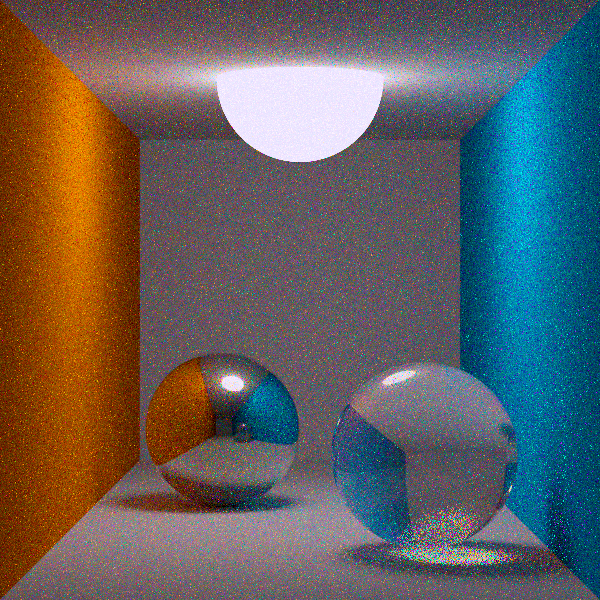
\includegraphics[width=0.4\textwidth]{images/Path_Tracing_Low.png}
        \hspace*{0.05\textwidth}
        \label{fig:closed-mesh-gender0}
    }
    \hspace*{0.1\textwidth}
    \subfloat[Rendering der Cornell Box mit  Pathtracing und vielen Samples]{
    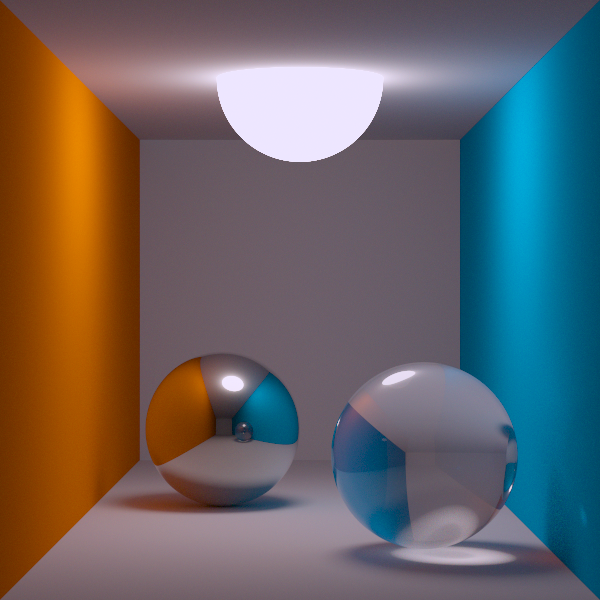
\includegraphics[width=0.4\textwidth]{images/Path_Tracing_High.png}
        \label{fig:closed-mesh-gender1}
    }
\end{figure}


\subsection{Monte Carlo Methode}
Die Monte Carlo Methode bezeichnet die Anwendung des  Gesetztes der großen Zahlen auf die Rendergleichung.


\subsubsection{Raymarching}
\subsection{Klassifikation der Verfahren}

\subsection{Datenstrukturen für Bereichsabfragen}


\subsection{Labor}
\subsubsection{Blender}
\subsubsection{Echtzeitfähiges Raymarching in WebGL}
